\documentclass[12pt, a4paper, oneside]{book}

\usepackage[left = 3cm, right = 2cm, top = 3cm, bottom = 3cm]{geometry}
\usepackage[dutch]{babel}
\usepackage{tikz}

\begin{document}

\textbf{\LARGE{Bomen in \LaTeX}}

\bigskip

\textbf{\Large{Gewortelde bomen}}

\bigskip

\begin{table}[htb!]
\centering
\begin{tabular}{ccc}
Orde & Gewortelde bomen & Aantal \\
\\
\hline
\\
$1$ & 
\begin{tikzpicture}[grow = up, level distance = 0.5cm, sibling distance = 1cm,
    every node/.style = {shape = circle, draw, fill = black, inner sep = 1pt}]
        \node {};
\end{tikzpicture} & $1$ \\
\\
$2$ &

\begin{tikzpicture}[grow = up, level distance = 0.5cm, sibling distance = 1cm,
    every node/.style = {shape = circle, draw, fill = black, inner sep = 1pt}]
        \node {}
            child[missing]{ node{} }
            child{ node{} };
\end{tikzpicture} & $1$ \\
\\
$3$ &
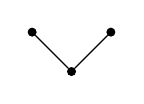
\begin{tikzpicture}[grow = up, level distance = 0.5cm, sibling distance = 1cm,
    every node/.style = {shape = circle, draw, fill = black, inner sep = 1pt}]
        \node {}
            child{ node{} }
            child{ node{} };
\end{tikzpicture}
\hspace{1cm}
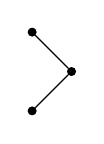
\begin{tikzpicture}[grow = up, level distance = 0.5cm, sibling distance = 1cm,
    every node/.style = {shape = circle, draw, fill = black, inner sep = 1pt}]
        \node {}
            child{ node{} 
                child[missing]{ node{} }
                child{ node{} }}
            child[missing]{ node{} };
\end{tikzpicture} & $2$ \\
\\
$4$ &
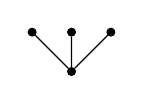
\begin{tikzpicture}[grow = up, level distance = 0.5cm, sibling distance = 0.5cm,
    every node/.style = {shape = circle, draw, fill = black, inner sep = 1pt}]
        \node {}
            child{ node{} }
            child{ node{} }
            child{ node{} };
\end{tikzpicture}
\hspace{1cm}
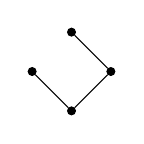
\begin{tikzpicture}[grow = up, level distance = 0.5cm, sibling distance = 1cm,
    every node/.style = {shape = circle, draw, fill = black, inner sep = 1pt}]
        \node {}
            child{ node {}
                child[missing]{ node{} }
                child{ node{} }}
            child{ node {}};
\end{tikzpicture}
\hspace{1cm}
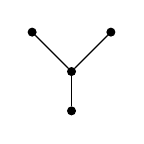
\begin{tikzpicture}[grow = up, level distance = 0.5cm, sibling distance = 1cm,
    every node/.style = {shape = circle, draw, fill = black, inner sep = 1pt}]
        \node {}
            child{ node {}
                child{ node{} }
                child{ node{} }};
\end{tikzpicture}
\hspace{1cm}
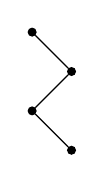
\begin{tikzpicture}[grow = up, level distance = 0.5cm, sibling distance = 1cm,
    every node/.style = {shape = circle, draw, fill = black, inner sep = 1pt}]
        \node {}
            child[missing]{ node{} }
            child{ node{} 
                child{ node{} 
                    child[missing]{ node{} }
                    child{ node{} }}
                child[missing]{ node{} }};
\end{tikzpicture} & $4$ \\
\\
\hline
\end{tabular}
\caption{Alle gewortelde bomen t.e.m.\ orde $4$.}
\end{table}

\begin{table}[htb!]
\centering
\begin{tabular}{c|c|c|c|c}
$t$ & $t_i$ & $t_j$ & $t_I$ & $t_J$ \\
\hline
& & & & \\
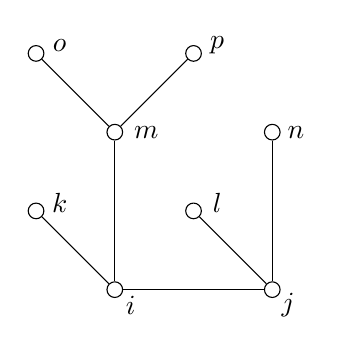
\begin{tikzpicture}
    \node [shape = circle, draw, inner sep = 2pt] (o) at (0,0) {};
    \node (O) at (0.3,0.1) {$o$};
    \node [shape = circle, draw, inner sep = 2pt] (p) at (2,0) {};
    \node (P) at (2.3,0.1) {$p$};
    \node [shape = circle, draw, inner sep = 2pt] (m) at (1,-1) {};
    \node (M) at (1.4,-1) {$m$};
    \node [shape = circle, draw, inner sep = 2pt] (n) at (3,-1) {};
    \node (N) at (3.3,-1) {$n$};
    \node [shape = circle, draw, inner sep = 2pt] (k) at (0,-2) {};
    \node (K) at (0.3,-1.9) {$k$};
    \node [shape = circle, draw, inner sep = 2pt] (l) at (2,-2) {};
    \node (L) at (2.3,-1.9) {$l$};
    \node [shape = circle, draw, inner sep = 2pt] (i) at (1,-3) {};
    \node (I) at (1.2,-3.2) {$i$};
    \node [shape = circle, draw, inner sep = 2pt] (j) at (3,-3) {};
    \node (J) at (3.2,-3.2) {$j$};
    
    \draw (o) to (m);
    \draw (p) to (m);
    \draw (k) to (i);
    \draw (m) to (i);
    \draw (l) to (j);
    \draw (n) to (j);
    \draw (i) to (j);
\end{tikzpicture}
&
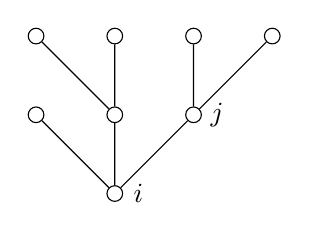
\begin{tikzpicture}[grow = up, level distance = 1cm, sibling distance = 1cm]
    \node [shape = circle, draw, inner sep = 2pt]{}
        child{ node[shape = circle, draw, inner sep = 2pt]{}
            child{ node[shape = circle, draw, inner sep = 2pt]{} }
            child{ node[shape = circle, draw, inner sep = 2pt]{} }
            child[missing]{ node{} }}
        child{ node[shape = circle, draw, inner sep = 2pt]{}
            child[missing]{ node{} }
            child{ node[shape = circle, draw, inner sep = 2pt]{} }
            child{ node[shape = circle, draw, inner sep = 2pt]{} }}
        child{ node[shape = circle, draw, inner sep = 2pt]{}};
    \node (I) at (0.3,0) {$i$};
    \node (J) at (1.3,1) {$j$};
\end{tikzpicture}
&
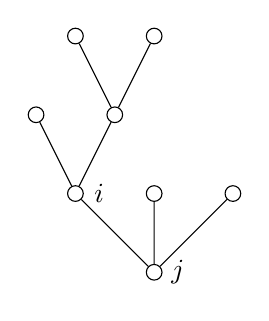
\begin{tikzpicture}[grow = up, level distance = 1cm, sibling distance = 1cm]
    \node [shape = circle, draw, inner sep = 2pt]{}
        child{ node[shape = circle, draw, inner sep = 2pt]{} }
        child{ node[shape = circle, draw, inner sep = 2pt]{} }
        child{ node[shape = circle, draw, inner sep = 2pt]{}
            child{ node[shape = circle, draw, inner sep = 2pt]{}
                child{ node[shape = circle, draw, inner sep = 2pt]{} }
                child{ node[shape = circle, draw, inner sep = 2pt]{} }}
            child{ node[shape = circle, draw, inner sep = 2pt]{} }};
    \node (J) at (0.3,0) {$j$};
    \node (I) at (-0.7, 1) {$i$};
\end{tikzpicture}
&
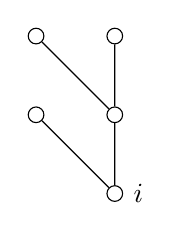
\begin{tikzpicture}[grow = up, level distance = 1cm, sibling distance = 1cm]
    \node [shape = circle, draw, inner sep = 2pt]{}
        child[missing]{ node{} }
        child{ node[shape = circle, draw, inner sep = 2pt]{}
            child[missing]{ node{} }
            child{ node[shape = circle, draw, inner sep = 2pt]{} }
            child{ node[shape = circle, draw, inner sep = 2pt]{} }}
        child{ node[shape = circle, draw, inner sep = 2pt]{}};
    \node (I) at (0.3,0) {$i$};
\end{tikzpicture}
&
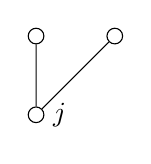
\begin{tikzpicture}[grow = up, level distance = 1cm, sibling distance = 1cm]
    \node [shape = circle, draw, inner sep = 2pt]{}
        child{ node[shape = circle, draw, inner sep = 2pt]{} }
        child{ node[shape = circle, draw, inner sep = 2pt]{} }
        child[missing]{ node{} };
    \node (J) at (0.3,0) {$j$};
\end{tikzpicture} \\
& & & & \\
\hline
\end{tabular}
\caption{Iets moeilijker.}
\end{table}

\newpage

\textbf{\Large{Tweekleurige gewortelde bomen}}

\begin{table}[htb!]
\centering
\begin{tabular}{ccc}
Orde & Tweekleurige gewortelde bomen & Aantal \\
\\
\hline
\\
$1$ & 
\begin{tikzpicture}[grow = up, level distance = 0.5cm, sibling distance = 1cm,
    every node/.style = {shape = circle, draw, fill = black, inner sep = 1pt}]
        \node {};
\end{tikzpicture}
\hspace{1cm}
\begin{tikzpicture}[grow = up, level distance = 0.5cm, sibling distance = 1cm,
    every node/.style = {shape = circle, draw, fill = white, inner sep = 1pt}]
        \node {};
\end{tikzpicture} & $2$ \\
\\
\hline
\\
$2$ &

\begin{tikzpicture}[grow = up, level distance = 0.5cm, sibling distance = 1cm,
    every node/.style = {shape = circle, draw, inner sep = 1pt}]
        \node[fill = black] {}
            child[missing]{ node{} }
            child{ node[fill = white]{} };
\end{tikzpicture}
\hspace{1cm}

\begin{tikzpicture}[grow = up, level distance = 0.5cm, sibling distance = 1cm,
    every node/.style = {shape = circle, draw, inner sep = 1pt}]
        \node[fill = white] {}
            child[missing]{ node{} }
            child{ node[fill = black]{} };
\end{tikzpicture} & $2$ \\
\\
\hline
\\
$3$ &
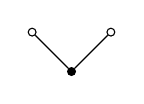
\begin{tikzpicture}[grow = up, level distance = 0.5cm, sibling distance = 1cm,
    every node/.style = {shape = circle, draw, inner sep = 1pt}]
        \node[fill = black] {}
            child{ node[fill = white]{} }
            child{ node[fill = white]{} };
\end{tikzpicture}
\hspace{1cm}
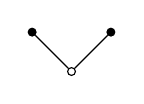
\begin{tikzpicture}[grow = up, level distance = 0.5cm, sibling distance = 1cm,
    every node/.style = {shape = circle, draw, inner sep = 1pt}]
        \node[fill = white] {}
            child{ node[fill = black]{} }
            child{ node[fill = black]{} };
\end{tikzpicture}
\hspace{1cm}
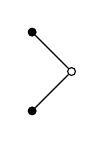
\begin{tikzpicture}[grow = up, level distance = 0.5cm, sibling distance = 1cm,
    every node/.style = {shape = circle, draw, inner sep = 1pt}]
        \node[fill = black] {}
            child{ node[fill = white]{} 
                child[missing]{ node{} }
                child{ node[fill = black]{} }}
            child[missing]{ node{} };
\end{tikzpicture}
\hspace{1cm}
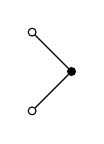
\begin{tikzpicture}[grow = up, level distance = 0.5cm, sibling distance = 1cm,
    every node/.style = {shape = circle, draw, inner sep = 1pt}]
        \node[fill = white] {}
            child{ node[fill = black]{} 
                child[missing]{ node{} }
                child{ node[fill = white]{} }}
            child[missing]{ node{} };
\end{tikzpicture} & $4$ \\
\\
\hline
\\
$4$ &
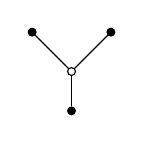
\begin{tikzpicture}[grow = up, level distance = 0.5cm, sibling distance = 1cm,
    every node/.style = {shape = circle, draw, inner sep = 1pt}]
        \node[fill = black] {}
            child { node[fill = white]{}
                child{ node[fill = black]{} }
                child{ node[fill = black]{} }};
\end{tikzpicture}
\hspace{1cm}
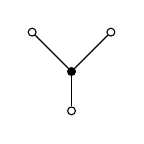
\begin{tikzpicture}[grow = up, level distance = 0.5cm, sibling distance = 1cm,
    every node/.style = {shape = circle, draw, inner sep = 1pt}]
        \node[fill = white] {}
            child { node[fill = black]{}
                child{ node[fill = white]{} }
                child{ node[fill = white]{} }};
\end{tikzpicture}
\hspace{1cm}
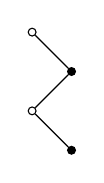
\begin{tikzpicture}[grow = up, level distance = 0.5cm, sibling distance = 1cm,
    every node/.style = {shape = circle, draw, inner sep = 1pt}]
        \node[fill = black] {}
            child[missing]{ node{} }
            child{ node[fill = white]{} 
                child{ node[fill = black]{} 
                    child[missing]{ node{} }
                    child{ node[fill = white]{} }}
                child[missing]{ node{} }};
\end{tikzpicture}
\hspace{1cm}
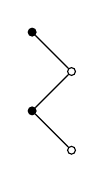
\begin{tikzpicture}[grow = up, level distance = 0.5cm, sibling distance = 1cm,
    every node/.style = {shape = circle, draw, inner sep = 1pt}]
        \node[fill = white] {}
            child[missing]{ node{} }
            child{ node[fill = black]{} 
                child{ node[fill = white]{} 
                    child[missing]{ node{} }
                    child{ node[fill = black]{} }}
                child[missing]{ node{} }};
\end{tikzpicture} & $8$ \\
& 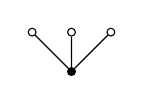
\begin{tikzpicture}[grow = up, level distance = 0.5cm, sibling distance = 0.5cm,
    every node/.style = {shape = circle, draw, inner sep = 1pt}]
        \node[fill = black] {}
            child{ node[fill = white]{} }
            child{ node[fill = white]{} }
            child{ node[fill = white]{} };
\end{tikzpicture}
\hspace{1cm}
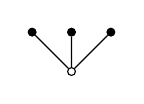
\begin{tikzpicture}[grow = up, level distance = 0.5cm, sibling distance = 0.5cm,
    every node/.style = {shape = circle, draw, inner sep = 1pt}]
        \node[fill = white] {}
            child{ node[fill = black]{} }
            child{ node[fill = black]{} }
            child{ node[fill = black]{} };
\end{tikzpicture}
\hspace{1cm}
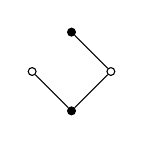
\begin{tikzpicture}[grow = up, level distance = 0.5cm, sibling distance = 1cm,
    every node/.style = {shape = circle, draw, inner sep = 1pt}]
        \node[fill = black] {}
            child { node[fill = white]{}
                child[missing]{ node{} }
                child{ node[fill = black]{} }}
            child { node[fill = white]{} };
\end{tikzpicture}
\hspace{1cm}
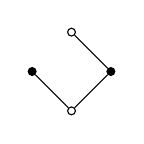
\begin{tikzpicture}[grow = up, level distance = 0.5cm, sibling distance = 1cm,
    every node/.style = {shape = circle, draw, inner sep = 1pt}]
        \node[fill = white] {}
            child { node[fill = black]{}
                child[missing]{ node{} }
                child{ node[fill = white]{} }}
            child { node[fill = black]{} };
\end{tikzpicture} & \\
\\
\hline
\end{tabular}
\caption{Alle tweekleurige gewortelde bomen t.e.m.\ orde $4$.}
\end{table}

\begin{table}[htb!]
\centering
\begin{tabular}{c|c|c|c|c}
$t$ & $t_i$ & $t_j$ & $t_I$ & $t_J$ \\
\hline
& & & & \\
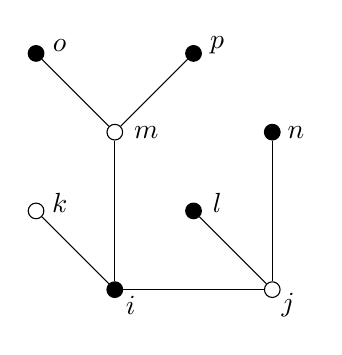
\begin{tikzpicture}
    \node [draw, shape = circle, fill = black, inner sep = 2pt] (o) at (0,0) {};
    \node (O) at (0.3,0.1) {$o$};
    \node [draw, shape = circle, fill = black, inner sep = 2pt] (p) at (2,0) {};
    \node (P) at (2.3,0.1) {$p$};
    \node [draw, shape = circle, inner sep = 2pt] (m) at (1,-1) {};
    \node (M) at (1.4,-1) {$m$};
    \node [draw, shape = circle, fill = black, inner sep = 2pt] (n) at (3,-1) {};
    \node (N) at (3.3,-1) {$n$};
    \node [draw, shape = circle, inner sep = 2pt] (k) at (0,-2) {};
    \node (K) at (0.3,-1.9) {$k$};
    \node [draw, shape = circle, fill = black, inner sep = 2pt] (l) at (2,-2) {};
    \node (L) at (2.3,-1.9) {$l$};
    \node [draw, shape = circle, fill = black, inner sep = 2pt] (i) at (1,-3) {};
    \node (I) at (1.2,-3.2) {$i$};
    \node [draw, shape = circle, inner sep = 2pt] (j) at (3,-3) {};
    \node (J) at (3.2,-3.2) {$j$};
    
    \draw (o) to (m);
    \draw (p) to (m);
    \draw (k) to (i);
    \draw (m) to (i);
    \draw (l) to (j);
    \draw (n) to (j);
    \draw (i) to (j);
\end{tikzpicture}
&
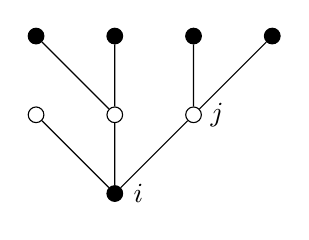
\begin{tikzpicture}[grow = up, level distance = 1cm, sibling distance = 1cm]
    \node [shape = circle, draw, fill = black, inner sep = 2pt]{}
        child{ node[shape = circle, draw, inner sep = 2pt]{}
            child{ node[shape = circle, draw, fill = black, inner sep = 2pt]{} }
            child{ node[shape = circle, draw, fill = black, inner sep = 2pt]{} }
            child[missing]{ node{} }}
        child{ node[shape = circle, draw, inner sep = 2pt]{}
            child[missing]{ node{} }
            child{ node[shape = circle, draw, fill = black, inner sep = 2pt]{} }
            child{ node[shape = circle, draw, fill = black, inner sep = 2pt]{} }}
        child{ node[shape = circle, draw, inner sep = 2pt]{}};
    \node (I) at (0.3,0) {$i$};
    \node (J) at (1.3,1) {$j$};
\end{tikzpicture}
&
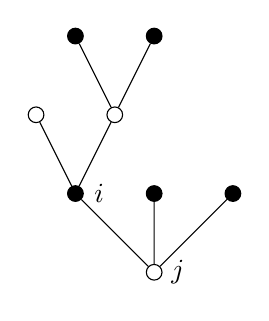
\begin{tikzpicture}[grow = up, level distance = 1cm, sibling distance = 1cm]
    \node [shape = circle, draw, inner sep = 2pt]{}
        child{ node[shape = circle, draw, fill = black, inner sep = 2pt]{} }
        child{ node[shape = circle, draw, fill = black, inner sep = 2pt]{} }
        child{ node[shape = circle, draw, fill = black, inner sep = 2pt]{}
            child{ node[shape = circle, draw, inner sep = 2pt]{}
                child{ node[shape = circle, draw, fill = black, inner sep = 2pt]{} }
                child{ node[shape = circle, draw, fill = black, inner sep = 2pt]{} }}
            child{ node[shape = circle, draw, inner sep = 2pt]{} }};
    \node (J) at (0.3,0) {$j$};
    \node (I) at (-0.7, 1) {$i$};
\end{tikzpicture}
&
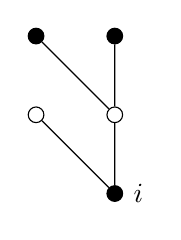
\begin{tikzpicture}[grow = up, level distance = 1cm, sibling distance = 1cm]
    \node [shape = circle, draw, fill = black, inner sep = 2pt]{}
        child[missing]{ node{} }
        child{ node[shape = circle, draw, inner sep = 2pt]{}
            child[missing]{ node{} }
            child{ node[shape = circle, draw, fill = black, inner sep = 2pt]{} }
            child{ node[shape = circle, draw, fill = black, inner sep = 2pt]{} }}
        child{ node[shape = circle, draw, inner sep = 2pt]{}};
    \node (I) at (0.3,0) {$i$};
\end{tikzpicture}
&
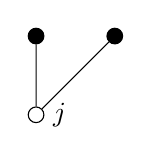
\begin{tikzpicture}[grow = up, level distance = 1cm, sibling distance = 1cm]
    \node [shape = circle, draw, inner sep = 2pt]{}
        child{ node[shape = circle, draw, fill = black, inner sep = 2pt]{} }
        child{ node[shape = circle, draw, fill = black, inner sep = 2pt]{} }
        child[missing]{ node{} };
    \node (J) at (0.3,0) {$j$};
\end{tikzpicture} \\
& & & & \\
\hline
\end{tabular}
\caption{Iets moeilijker.}
\end{table}

\newpage

\textbf{\Large{Speciale gewortelde bomen}}

\begin{table}[htb!]
\centering
\begin{tabular}{ccc}
Orde & Speciale gewortelde bomen & Aantal \\
\\
\hline
\\
$1$ & 

\begin{tikzpicture}[grow = up, level distance = 0.5cm, sibling distance = 1cm,
    every node/.style = {shape = circle, draw, fill = black, inner sep = 2pt}]
        \node {};
\end{tikzpicture} & $1$ \\
\\
$2$ &

\begin{tikzpicture}[grow = up, level distance = 0.5cm, sibling distance = 1cm,
    every node/.style = {shape = circle, draw, fill = black}]
        \node[inner sep = 2pt] {}
            child[missing]{ node{} }
            child{ node[inner sep = 1pt]{} };
\end{tikzpicture} & $1$ \\
\\
$3$ &
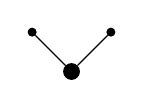
\begin{tikzpicture}[grow = up, level distance = 0.5cm, sibling distance = 1cm,
    every node/.style = {shape = circle, draw, fill = black}]
        \node[inner sep = 2pt] {}
            child{ node[inner sep = 1pt]{} }
            child{ node[inner sep = 1pt]{} };
\end{tikzpicture}
\hspace{1cm}
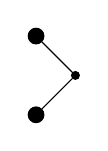
\begin{tikzpicture}[grow = up, level distance = 0.5cm, sibling distance = 1cm,
    every node/.style = {shape = circle, draw, fill = black}]
        \node[inner sep = 2pt] {}
            child{ node[inner sep = 1pt]{} 
                child[missing]{ node{} }
                child{ node[inner sep = 2pt]{} }}
            child[missing]{ node{} };
\end{tikzpicture} & $2$ \\
\\
$4$ &
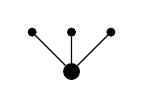
\begin{tikzpicture}[grow = up, level distance = 0.5cm, sibling distance = 0.5cm,
    every node/.style = {shape = circle, draw, fill = black}]
        \node[inner sep = 2pt] {}
            child{ node[inner sep = 1pt]{} }
            child{ node[inner sep = 1pt]{} }
            child{ node[inner sep = 1pt]{} };
\end{tikzpicture}
\hspace{1cm}
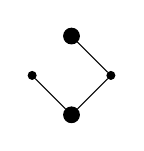
\begin{tikzpicture}[grow = up, level distance = 0.5cm, sibling distance = 1cm,
    every node/.style = {shape = circle, draw, fill = black}]
        \node[inner sep = 2pt] {}
            child { node[inner sep = 1pt]{}
                child[missing]{ node{} }
                child{ node[inner sep = 2pt]{} }}
            child { node[inner sep = 1pt]{}};
\end{tikzpicture}
\hspace{1cm}
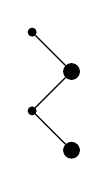
\begin{tikzpicture}[grow = up, level distance = 0.5cm, sibling distance = 1cm,
    every node/.style = {shape = circle, draw, fill = black}]
        \node[inner sep = 2pt] {}
            child[missing]{ node{} }
            child{ node[inner sep = 1pt]{} 
                child{ node[inner sep = 2pt]{} 
                    child[missing]{ node{} }
                    child{ node[inner sep = 1pt]{} }}
                child[missing]{ node{} }};
\end{tikzpicture} & $3$ \\
\\
\hline
\end{tabular}
\caption{Alle speciale gewortelde bomen t.e.m.\ orde 4.}
\end{table}

\begin{table}[htb!]
\centering
\begin{tabular}{c|c|c|c|c|c}
$t_i$ & $t_j$ & $t_I$ & $t_J$ & $t^I$ & $t^J$ \\
\hline
& & & & & \\
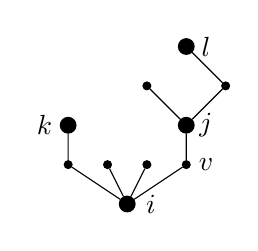
\begin{tikzpicture}[grow = up, level distance = 0.5cm, sibling distance = 0.5cm]
    \node[shape = circle, draw, fill = black, inner sep = 2pt] {}
        child{ node[shape = circle, draw, fill = black, inner sep = 1pt]{} 
            child{ node[shape = circle, draw, fill = black, inner sep = 2pt]{}
                child{ node[shape = circle, draw, fill = black, inner sep = 1pt]{}
                    child[missing]{ node{} }
                    child[missing]{ node{} }
                    child{ node[shape = circle, draw, fill = black, inner sep = 2pt]{} }}
                child[missing]{ node{} }
                child{ node[shape = circle, draw, fill = black, inner sep = 1pt]{} }}}
        child{ node[shape = circle, draw, fill = black, inner sep = 1pt]{} }
        child{ node[shape = circle, draw, fill = black, inner sep = 1pt]{} }
        child{ node[shape = circle, draw, fill = black, inner sep = 1pt]{} 
            child{ node[shape = circle, draw, fill = black, inner sep = 2pt]{}}};
    \node (I) at (0.3,0) {$i$};
    \node (J) at (1,1) {$j$};
    \node (K) at (-1.05, 1) {$k$};
    \node (L) at (1,2) {$l$};
    \node (V) at (1,0.5) {$v$};
\end{tikzpicture}
&
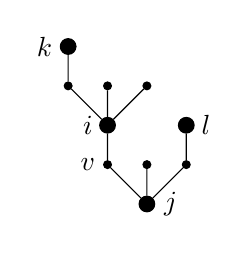
\begin{tikzpicture}[grow = up, level distance = 0.5cm, sibling distance = 0.5cm]
    \node[shape = circle, draw, fill = black, inner sep = 2pt] {}
        child{ node[shape = circle, draw, fill = black, inner sep = 1pt]{}
            child{ node[shape = circle, draw, fill = black, inner sep = 2pt]{} }}
        child{ node[shape = circle, draw, fill = black, inner sep = 1pt]{} }
        child{ node[shape = circle, draw, fill = black, inner sep = 1pt]{}
            child{ node[shape = circle, draw, fill = black, inner sep = 2pt]{}
                child{ node[shape = circle, draw, fill = black, inner sep = 1pt]{} }
                child{ node[shape = circle, draw, fill = black, inner sep = 1pt]{} }
                child{ node[shape = circle, draw, fill = black, inner sep = 1pt]{}
                    child{ node[shape = circle, draw, fill = black, inner sep = 2pt]{} }}}};
    \node (J) at (0.3,0) {$j$};
    \node (I) at (-0.75,1) {$i$};
    \node (K) at (-1.3,2) {$k$};
    \node (L) at (0.75,1) {$l$};
    \node (V) at (-0.75,0.5) {$v$};
\end{tikzpicture}
&
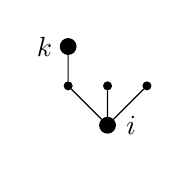
\begin{tikzpicture}[grow = up, level distance = 0.5cm, sibling distance = 0.5cm]
    \node[shape = circle, draw, fill = black, inner sep = 2pt] {}
        child{ node[shape = circle, draw, fill = black, inner sep = 1pt]{} }
        child{ node[shape = circle, draw, fill = black, inner sep = 1pt]{} }
        child{ node[shape = circle, draw, fill = black, inner sep = 1pt]{} 
            child{ node[shape = circle, draw, fill = black, inner sep = 2pt]{}}};
    \node (I) at (0.3,0) {$i$};
    \node (K) at (-0.8,1) {$k$};
\end{tikzpicture}
&
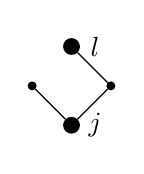
\begin{tikzpicture}[grow = up, level distance = 0.5cm, sibling distance = 1cm]
    \node[shape = circle, draw, fill = black, inner sep = 2pt] {}
        child { node[shape = circle, draw, fill = black, inner sep = 1pt]{}
            child[missing]{ node{} }
            child{ node[shape = circle, draw, fill = black, inner sep = 2pt]{} }}
        child { node[shape = circle, draw, fill = black, inner sep = 1pt]{}};
    \node (J) at (0.3,0) {$j$};
    \node (L) at (0.3,1) {$l$};
\end{tikzpicture}
&
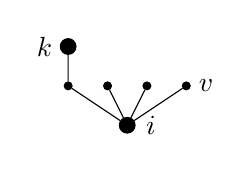
\begin{tikzpicture}[grow = up, level distance = 0.5cm, sibling distance = 0.5cm]
    \node[shape = circle, draw, fill = black, inner sep = 2pt] {}
        child{ node[shape = circle, draw, fill = black, inner sep = 1pt]{} }
        child{ node[shape = circle, draw, fill = black, inner sep = 1pt]{} }
        child{ node[shape = circle, draw, fill = black, inner sep = 1pt]{} }
        child{ node[shape = circle, draw, fill = black, inner sep = 1pt]{} 
            child{ node[shape = circle, draw, fill = black, inner sep = 2pt]{}}};
    \node (I) at (0.3,0) {$i$};
    \node (K) at (-1.05,1) {$k$};
    \node (V) at (1,0.5) {$v$};
\end{tikzpicture}
&
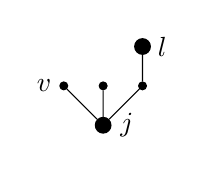
\begin{tikzpicture}[grow = up, level distance = 0.5cm, sibling distance = 0.5cm]
    \node[shape = circle, draw, fill = black, inner sep = 2pt] {}
        child{ node[shape = circle, draw, fill = black, inner sep = 1pt]{}
            child{ node[shape = circle, draw, fill = black, inner sep = 2pt]{} }}
        child{ node[shape = circle, draw, fill = black, inner sep = 1pt]{} }
        child{ node[shape = circle, draw, fill = black, inner sep = 1pt]{}};
    \node (J) at (0.3,0) {$j$};
    \node (L) at (0.75,1) {$l$};
    \node (V) at (-0.75,0.5) {$v$};
\end{tikzpicture}
\\
& & & & & \\
\hline
\end{tabular}
\caption{Iets moeilijker.}
\end{table}

\end{document}